\chapter{Missions complémentaires}
\label{chap:troisiemechapitre}

\section{Le projet MATRIX}

\subsection{Contexte du projet}

En plus de ma mission principale (participer aux développement de PPIL), j'ai travaillé sur le projet MATRIX. Nous avons formé une équipe de 6 stagiaires et nous nous sommes réparti différents rôles : CP(1), RF(1), RT(1), BA(2), SB(2). Mon rôle pour ce projet est celui de SB (développeur). Nous avons tous travaillé ensemble sur les différentes phases du projet. Et surtout (pour le moment) sur les phases de relation client, cadrage et conception. Dès que nous aurons fini les phases de cadrage et conception, nous allons commencer à développer. Le temps alloué pour ce projet est d'une demi-journée minimum par semaine.
 
\subsection{Étude des besoins (phase de cadrage)}

Nous avons eu une démarche de compréhension du client. Les managers de projet ont besoin de chercher des collaborateurs en fonction des compétences de ceux-ci pour créer leurs équipes.

\subsubsection{L'importance d'étudier les outils existants}

Pour réaliser cette tâche de recherche de collaborateurs répondant à certaines compétences, les managers de projets ont des outils / processus déjà existant, tels que :

Le premier outil utilisé au niveau du pôle CNAM métier étant un fichier Excel qui répertorie les compétences des collaborateurs. Cette solution pose des difficultés principalement au niveau de la maintenabilité des informations à jour.

La deuxième solution qui s'offre aux managers de projet est, dans l'intranet du groupe (tout Sopra Steria), une section de recherche d'expert en fonction d'une compétence. Cet outil ne répertorie qu'une partie des collaborateurs (les experts dans un domaine), et la localisation de ceux-ci n'est pas à jour.

\begin{figure}[!h]
\centering
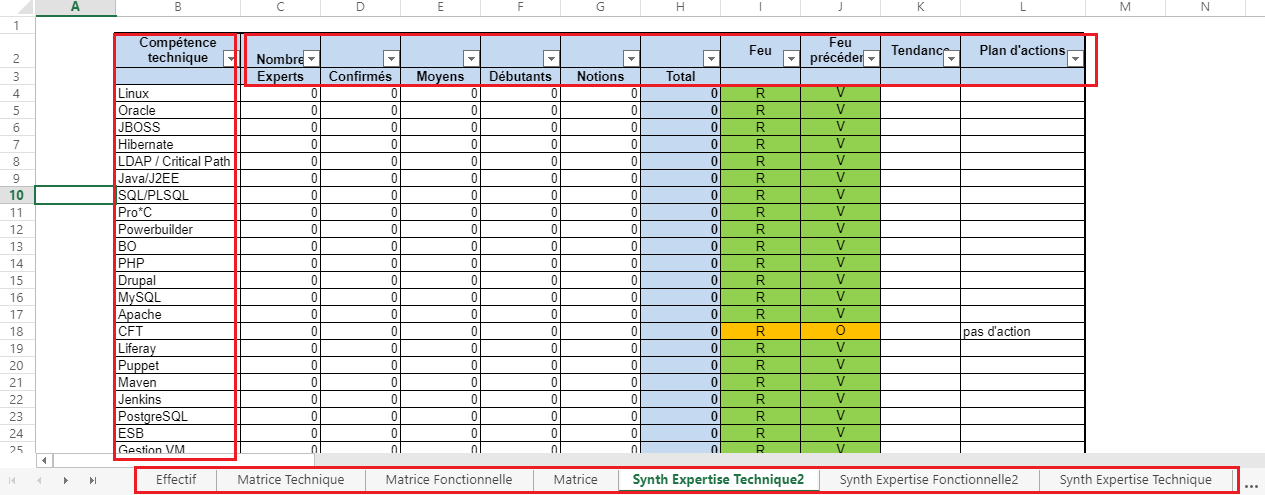
\includegraphics[width=1\textwidth]{images/MATRIX-excel.png}
\caption{MATRIX : Template du document Excel qui recense les collaborateurs en fonction de leurs compétences}
\end{figure}

Il est important d'analyser ce document car c'est celui-ci, qui dans la pratique est utilisé par les managers de projets. Pour la conception de notre application, il est important de prendre en compte la façon dont les informations sont agencées dans ce fichier Excel.

Aux vues des outils et processus cités ci-dessus, on voit bien que l'application MATRIX a sa place au sein du pôle CNAM métier et qu'elle serait un réel atout pour les managers de projets.

\subsection{Concevoir une application, notre démarche}

Lors de la conception de l'application, nous nous sommes retrouvés face à diverses problématiques. 

Par exemple, lorsque nous nous sommes demandés comment sera géré la liste des compétences en base de données : qui et comment seront ajoutées les compétences ?

Nous nous sommes retrouvés face à plusieurs questions : Est-ce qu'un utilisateur peut ajouter lui-même une fonctionnalité ? Ou bien est-ce qu'elle sont déterminées en base de données ? Si elles sont déterminées en base de données, comment en ajouter une nouvelle ? Faut-il faire des demandes administrateur ? Est-ce que les détails de la compétence (image, version) seront transmises avec ?

Toutes ces questions, nous avons pu y répondre, grâce à :
\begin{itemize}
\item l'étude des outils existants (document Excel) ;
\item différents points avec le client ;
\item priorité et faisabilité des fonctionnalités en un temps déterminé.
\end{itemize}

Nous avons choisi de :
\begin{itemize}
\item Ne pas prendre en compte les différentes versions des technologies (grâce au document Excel) ; 
\item Ne pas passer par l'administrateur pour ajouter une technologie (grâce aux entretiens avec le client) ;
\item Créer une liste par défaut des technologies en base de données (grâce au document Excel).
\end{itemize}


\subsubsection{Classer les fonctionnalités par priorité : Lot 1 et Lot 2}

Nous avons décidé que le lot 1 concernera les fonctionnalités principales et le lot 2 les fonctionnalités secondaires. Nous avons priorisé les fonctionnalités selon les besoins du client.

\subsubsection{Choix des technologies}

Nous avons été libre de choisir les technologies : 
\begin{itemize}
\item Java Spring 
\item JHipster 
\item JavaScript
\end{itemize}

Spring est un socle pour le développement d'applications très répandu en entreprise. Il représente un réel avantage en nous fournissant de nombreuses fonctionnalités qui peuvent être utilisées de plusieurs manières : ceci laisse le choix au développeur d'utiliser la solution qui correspond le plus à ses besoins.
Spring est ainsi un des frameworks le plus répandu dans le monde Java et dispose d'une grande popularité.

JHipster fournit des outils pour générer un projet avec côté client un frontal Web adaptatif (avec Angular et Bootstrap). JHipster nous permet d'atteindre nos objectif, avec plus de productivité et de qualité.

JavaScript, est le grand incontournable des pages web interactives. JHipster étant lui-même construit en parti en Angular (framework JavaScript).

\subsubsection{Mise en place des STD}

\subsubsection{Les maquettes}

Nous avons réalisé des maquettes du projet MATRIX en nous basant sur celles déjà existantes en les adaptant aux besoins du client. Ci-dessous voici deux des 7 maquettes.

\begin{figure}[!h]
\centering
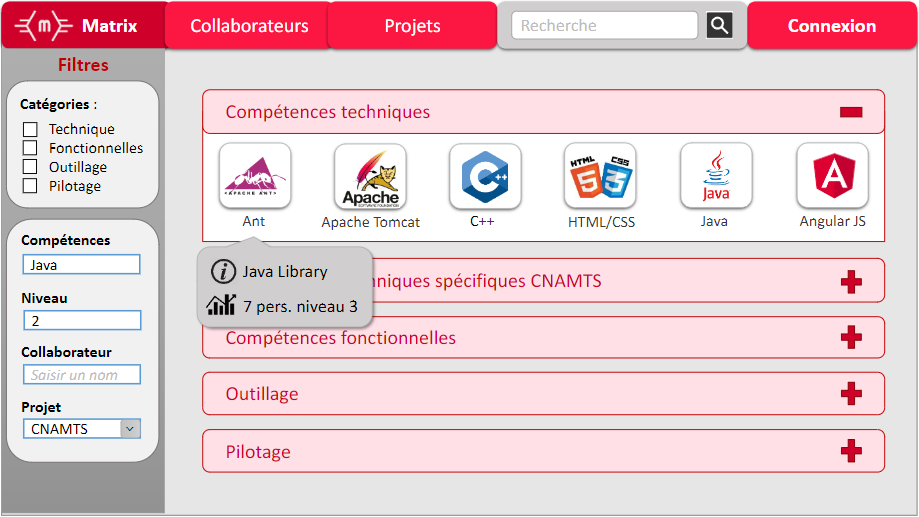
\includegraphics[width=1\textwidth]{images/matrix-maquette.png}
\caption{MATRIX : Maquette de recherche par compétence}
\end{figure}

\subsubsection{La base de données}

Voici la base de données du projet :
\begin{figure}[H]
\centering
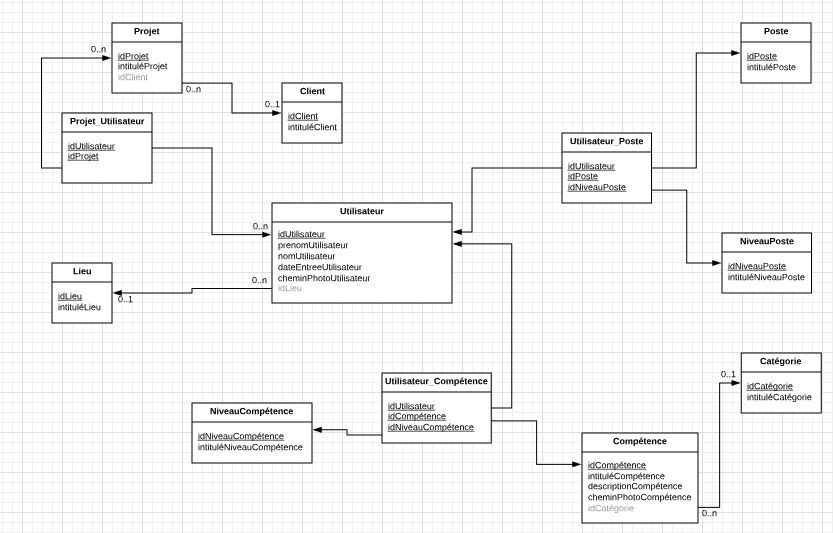
\includegraphics[width=0.8\textwidth]{images/matrix-bdd.png}
\caption{MATRIX : MCD}
\end{figure}

\subsection{Phase de développement}

\subsubsection{Installation de l’environnement}
Nous avons choisi d'utiliser l'IDE Intellij et GitLab afin de gérer nos dépots Git. Nous avons réalisé des tutoriels d'installation de nos environnements.

Nous commencerons nos développements dès que la phase de conception se terminera.

\subsection{Mise en place des SFG, STD}

Nous avons rédigé les spécifications fonctionnelles et les spécifications techniques en prenant en compte les différents lots. 

\section{Interview et présentation du métier de Business Analyste en vidéo}

Sopra Steria a proposé de réaliser une vidéo de présentation du métier de BA. Cette vidéo est destinée à présenter le métier aux nouveaux arrivants sur le pôle. Nous avons réalisé cette mission à trois. Nous avons pris l'initiative de réaliser des interview filmées de 3 collaborateurs. En parallèle, nous avons créé une animation sur l'outil Powtoon. Puis nous avons réalisé un montage vidéo en fusionnant les interview et l'animation Powtoon. Cette vidéo a été présentée à tous les acteurs du pôle CNAM Métier (plus de 100 personnes). La vidéo a été très appréciée. Cette mission a été l'occasion de découvrir le métier et d'échanger avec des collaborateurs expérimentés.

\begin{figure}[H]
\centering

\includegraphics[width=0.5\textwidth]{images/presBA.png}
\caption{Sopra Steria : Présentation du métier de BA}
\end{figure}
%%% Local Variables: 
%%% mode: latex
%%% TeX-master: "isae-report-template"
%%% End: 